
%(BEGIN_QUESTION)
% Copyright 2011, Tony R. Kuphaldt, released under the Creative Commons Attribution License (v 1.0)
% This means you may do almost anything with this work of mine, so long as you give me proper credit

A design team recommends the following control strategy for regulating liquid level in this process vessel:

$$\includegraphics[width=15.5cm]{i01821x01.eps}$$

Explain why this control strategy {\it cannot} work, and re-design it so that it can.

\vfil

\underbar{file i01821}
\eject
%(END_QUESTION)





%(BEGIN_ANSWER)

This is a graded question -- no answers or hints given!

%(END_ANSWER)





%(BEGIN_NOTES)

The fundamental principle to keep in mind for this problem is {\it mass balance}.  The only way to influence the liquid level in a vessel is to alter the balance of mass flow in versus mass flow out.  The control valve shown here fails to do that: it causes a certain mass flow rate to exit the vessel and then go right back in, for zero net effect.

Connecting the LIC to at least one of the valves going in or out of the vessel would make this a work-able system.

%INDEX Basics, control loop troubleshooting: determining reason a control strategy cannot work

%(END_NOTES)


